\documentclass{elegantbook}
\usepackage[square,numbers,sort&compress]{natbib}
\newcommand{\upcite}[1]{\textsuperscript{\textsuperscript{\cite{#1}}}}
\usepackage{multirow}
\usepackage{color}
\usepackage{tikz}
\usepackage{algorithm}
\usepackage{algorithmic}
\renewcommand{\algorithmicrequire}{ \textbf{Input:}} 
\renewcommand{\algorithmicensure}{ \textbf{Output:}} 
\usetikzlibrary{shapes.geometric, arrows}
\tikzstyle{startstop} = [rectangle, rounded corners, minimum width = 2cm, minimum height=1cm,text centered, draw = black, fill = red!40]
\tikzstyle{acti} = [rectangle, trapezium left angle=70, trapezium right angle=110, minimum width=5cm, minimum height=0.5cm, text centered, draw=black, fill = blue!40]
\tikzstyle{pool} = [rectangle, trapezium left angle=70, trapezium right angle=110, minimum width=2cm, minimum height=0.5cm, text centered, draw=black, fill = purple!40]
\tikzstyle{process} = [rectangle, minimum width=3cm, minimum height=1cm, text centered, draw=black, fill = green!50]
\tikzstyle{conv} = [rectangle, minimum width=3cm, minimum height=1cm, text centered, draw=black, fill = magenta!50]
\tikzstyle{loss} = [rectangle, rounded corners, minimum width = 2cm, minimum height=1cm,text centered, draw = black, fill = yellow!40]
\tikzstyle{arrow} = [->,>=stealth]

% title info
\title{Deep Learning}
\subtitle{MNIST Digits Classification with CNN}
% bio info
\author{Yantian Luo}
\institute{Electronic Engineering}
\version{2018310742}
\date{\today}
\logo{logo.png}
\cover{cover.jpg}

\begin{document}

\maketitle
\tableofcontents
\mainmatter
\hypersetup{pageanchor=true}
% add preface chapter here if needed
\chapter{Introduction}
MNIST digits dataset is a widely used database for image classification in machine learning field. It contains 60,000 training samples and 10,000 testing samples. Each sample is a $784\times1$ column vector, which is transformed from an original $28\times28$ pixels grayscale image.

In this homework, we will continue working on MNIST digits classification problem by utilizing Pytorch framework to implement neural networks. Pytorch provides good abstraction for different modules, and its auto-differentiation feature can save us from the backward details.

\chapter{Algorithm Design}
In the last two homework, we have implement Linear layer, activation layer, convolution layer and loss layer, in this homework, we only implement an important technique discovered recently and utilize Pytorch framework to implement others.

\section{Training phase}
For every input $x_i$ across a mini-batch, the output can be computed as :
\begin{equation}
BN(x_i)=\gamma \cdot \frac{x_i-\mu_B}{\sqrt{\sigma^2+\epsilon}}+\beta
\end{equation}
where $\gamma$ and $\beta$ are learnable parameters, $\mu_B$ is the mean of the mini-batch and $\sigma^2$ is the variance of the mini-batch.

\section{Evaluation phase}
When we test our samples one by one, the normalization may not work because we don’t have mini- batch concept this time. Therefore, during training we should keep running estimates of its computed mean and variance, which are then used for normalization during evaluation. The running estimates are kept with a default momentum of 0.9, which can be mathematically expressed as
\begin{equation}
\begin{aligned}
\hat{\mu}_{new} &= momentum \times \hat{\mu} + (1-momentum)\times \mu_t \\
\hat{\sigma}_{new}^2 &= momentum \times \hat{\sigma}^2 + (1-momentum)\times \sigma_t^2
\end{aligned}
\end{equation}
where where $\hat{\mu},\hat{\sigma}^2$ are the estimated statistic and $\mu_t,\sigma_t^2$ is the new observed value. 

\section{Results}
\begin{figure}[htbp]
	\centering
	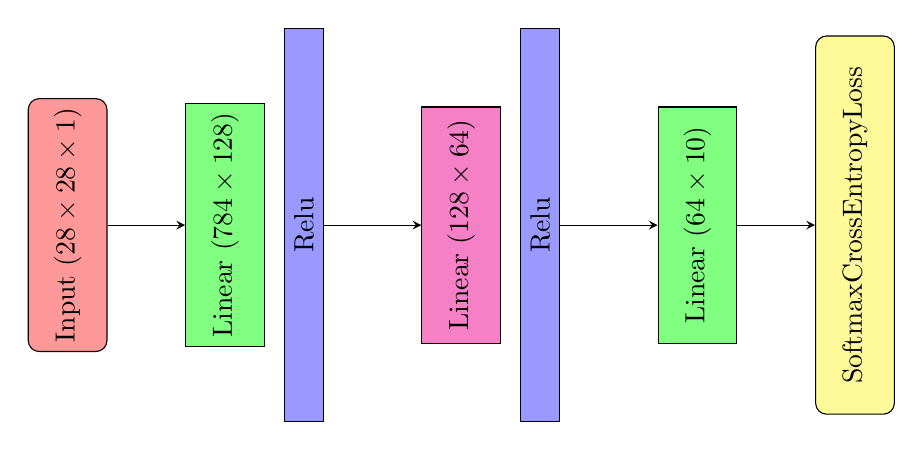
\begin{tikzpicture}
	\node (start) [startstop, rotate=90] {Input ($28\times28\times 1$)};
	\node (linear1) [process, rotate=90, below of=start, yshift=-1cm] {Linear ($784\times 128$)};
	\node (acti1) [acti, rotate=90, below of=linear1] {Relu};
	\node (linear2) [conv, rotate=90, below of=acti1, yshift=-1cm] {Linear ($128\times 64$)};
	\node (acti2) [acti, rotate=90, below of=linear2] {Relu};
	\node (linear3) [process, rotate=90, below of=acti2, yshift=-1cm] {Linear ($64\times 10$)};
	\node (loss) [loss, rotate=90, below of=linear3, yshift=-1cm, text width=13em] {SoftmaxCrossEntropyLoss};
	
	\draw [arrow](start) -- (linear1);
	%		\draw [arrow](conv1) -- (acti1);
	%		\draw [arrow](acti1) -- (pool1);
	\draw [arrow](acti1) -- (linear2);
	%		\draw [arrow](conv2) -- (acti2);
	%		\draw [arrow](acti2) -- (pool2);
	\draw [arrow](acti2) -- (linear3);
	\draw [arrow](linear3) -- (loss);
	\end{tikzpicture}
	\caption{\label{fig1}MLP Network Structure}
\end{figure}
\end{document}